\documentclass[aspectratio=169]{beamer}
\usepackage[utf8]{inputenc}
\usepackage{amsmath}
\usepackage{amsfonts}
\usepackage{amssymb}
\usepackage{graphicx}
\usepackage{booktabs}
\usepackage{multirow}
\usepackage{xcolor}
\usepackage{tikz}
\usepackage{hyperref}

\usetheme{Madrid}
\usecolortheme{default}

% Custom colors
\definecolor{primaryblue}{RGB}{0,102,204}
\definecolor{accentorange}{RGB}{255,102,0}
\definecolor{lightgray}{RGB}{240,240,240}

\setbeamercolor{title}{fg=primaryblue}
\setbeamercolor{frametitle}{fg=primaryblue}
\setbeamercolor{structure}{fg=primaryblue}

\title[LLM Performance in Taboo Games: Midterm Progress]{Evaluating Large Language Model Performance in Taboo Word Games: Midterm Progress Report}
\subtitle{MSc Computer Science - Research Project}
\author{Student Name}
\institute{University Name}
\date{\today}

\begin{document}

% Title slide
\begin{frame}
\titlepage
\end{frame}

% Table of contents
\begin{frame}{Presentation Outline}
\tableofcontents
\end{frame}

%==============================================
% 1. Project Overview & Background
%==============================================
\section{Project Overview \& Background}

% Section title slide
\begin{frame}
\begin{center}
\Huge \textbf{Project Overview \& Background}
\end{center}
\end{frame}

\begin{frame}{Research Motivation}
\begin{block}{Why Taboo Games for LLM Evaluation?}
\begin{itemize}
    \item \textbf{Constrained Communication}: Tests forbidden word avoidance
    \item \textbf{Creative Language Use}: Requires linguistic flexibility
    \item \textbf{Multi-dimensional Assessment}: Evaluates understanding and creativity
\end{itemize}
\end{block}

\begin{block}{Current Evaluation Limitations}
\begin{itemize}
    \item Traditional benchmarks focus on classification
    \item Limited creative generation assessment
    \item Lack of constraint-following evaluation
\end{itemize}
\end{block}

\begin{alertblock}{Research Innovation}
First comprehensive Taboo game evaluation framework for LLMs
\end{alertblock}
\end{frame}

\begin{frame}{Research Questions \& Objectives}
\begin{block}{Primary Research Questions}
\begin{enumerate}
    \item How do different LLMs perform in constrained communication?
    \item What factors influence Taboo game success?
    \item Do "thinking" models outperform traditional models?
    \item What linguistic features affect performance?
\end{enumerate}
\end{block}

\begin{block}{Project Objectives}
\begin{itemize}
    \item Develop comprehensive Taboo evaluation framework
    \item Compare 4 state-of-the-art LLMs
    \item Analyze linguistic features impact
    \item Identify optimal constrained generation strategies
\end{itemize}
\end{block}
\end{frame}

%==============================================
% 2. Methodology
%==============================================
\section{Methodology}

% Section title slide
\begin{frame}
\begin{center}
\Huge \textbf{Methodology}
\end{center}
\end{frame}

\begin{frame}{Experimental Design}
\begin{columns}[c]
\begin{column}{0.5\textwidth}
\begin{block}{Experimental Setup}
\begin{itemize}
    \item \textbf{Models}: 4 LLMs
    \begin{itemize}
        \item Claude Sonnet 4
        \item GPT-4o
        \item Gemini 2.5 Pro
        \item DeepSeek Chat V3
    \end{itemize}
    \item \textbf{Dataset}: 300 words
    \item \textbf{Games}: 4,800 total
    \item \textbf{Structure}: Max 4 turns
\end{itemize}
\end{block}
\end{column}

\begin{column}{0.48\textwidth}
\begin{center}
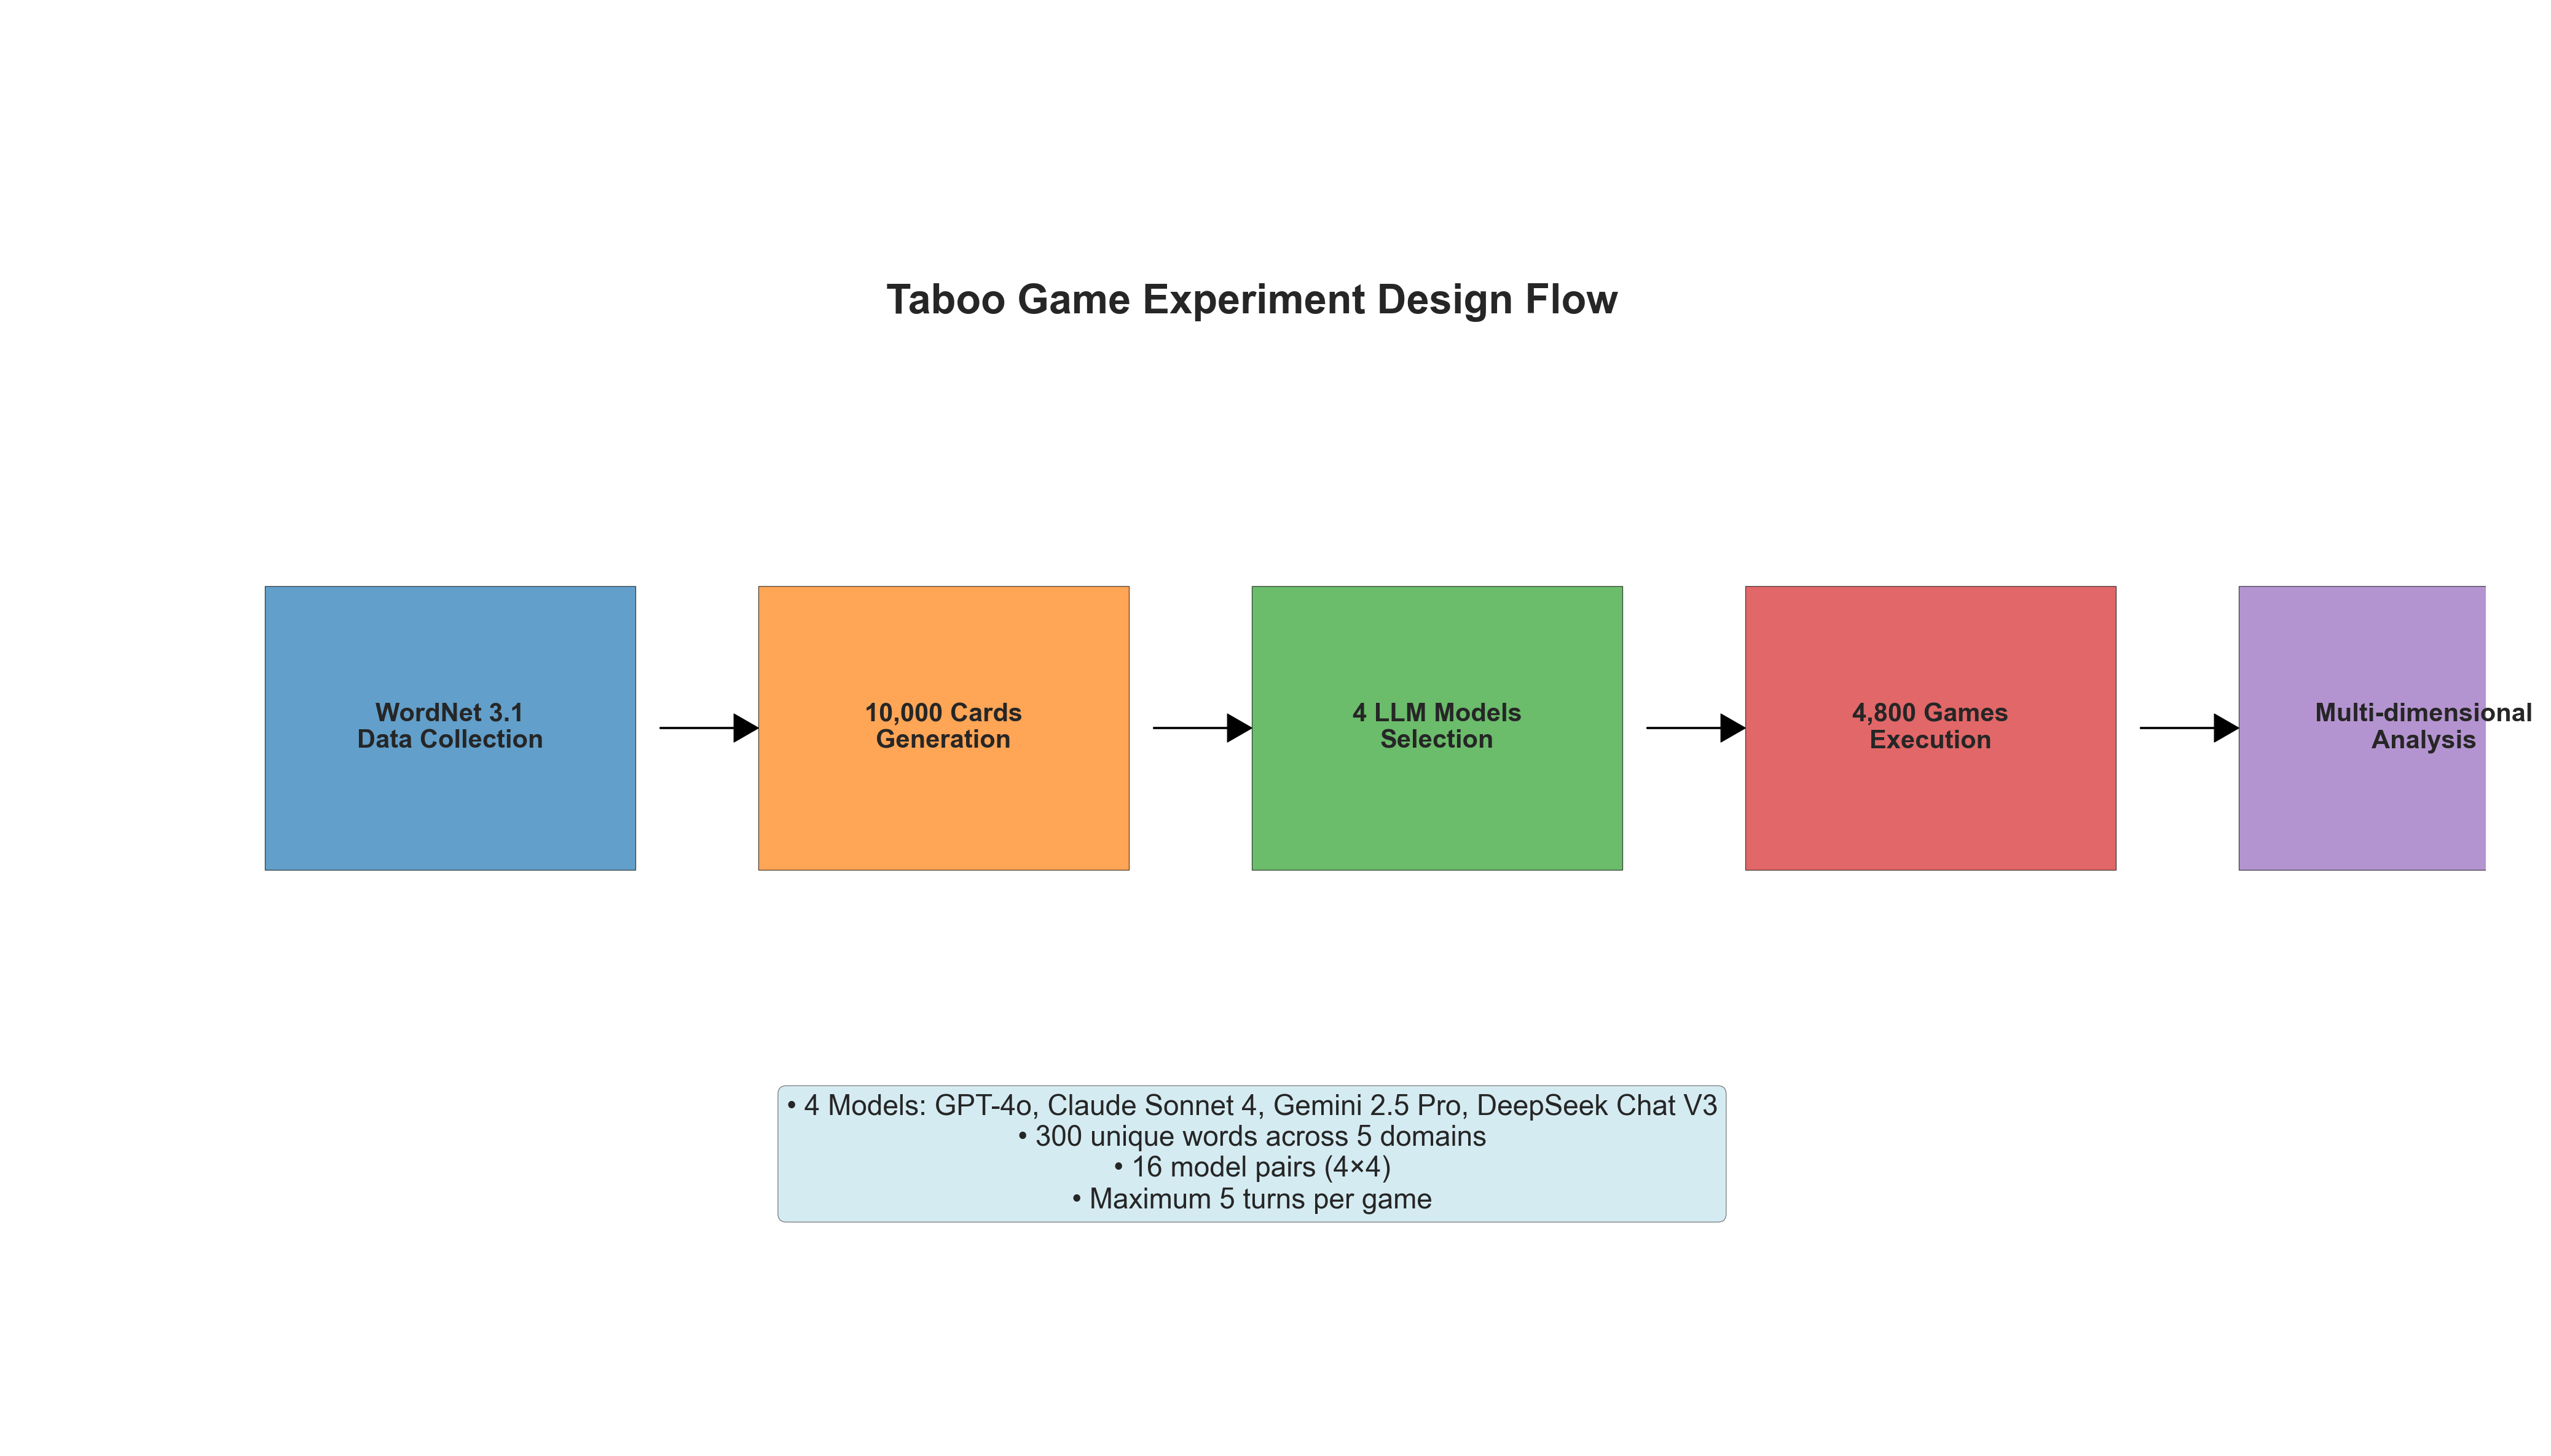
\includegraphics[width=\textwidth]{presentation_figures/figure1_flowchart.png}
\end{center}
\end{column}
\end{columns}
\end{frame}

\begin{frame}{Dataset Construction}
\begin{columns}[c]
\begin{column}{0.5\textwidth}
\begin{block}{Specialized Terms (200 words)}
\small
\begin{itemize}
    \item \textbf{Hard Science-Pure}: Chemistry (50)
    \item \textbf{Hard Science-Applied}: Computer Science (50)
    \item \textbf{Soft Science-Applied}: Finance (50)
    \item \textbf{Soft Science-Pure}: Philosophy (50)
    \item \textbf{General}: Common vocabulary (100)
\end{itemize}
\end{block}

\begin{block}{Data Sources}
\tiny
\begin{itemize}
    \item IUPAC Gold Book (Chemistry)
    \item Ada CS Glossary (Computer Science)
    \item Investopedia Dictionary (Finance)
    \item Stanford Encyclopedia (Philosophy)
    \item Manual cleaning and validation
\end{itemize}
\end{block}
\end{column}

\begin{column}{0.48\textwidth}
\begin{center}
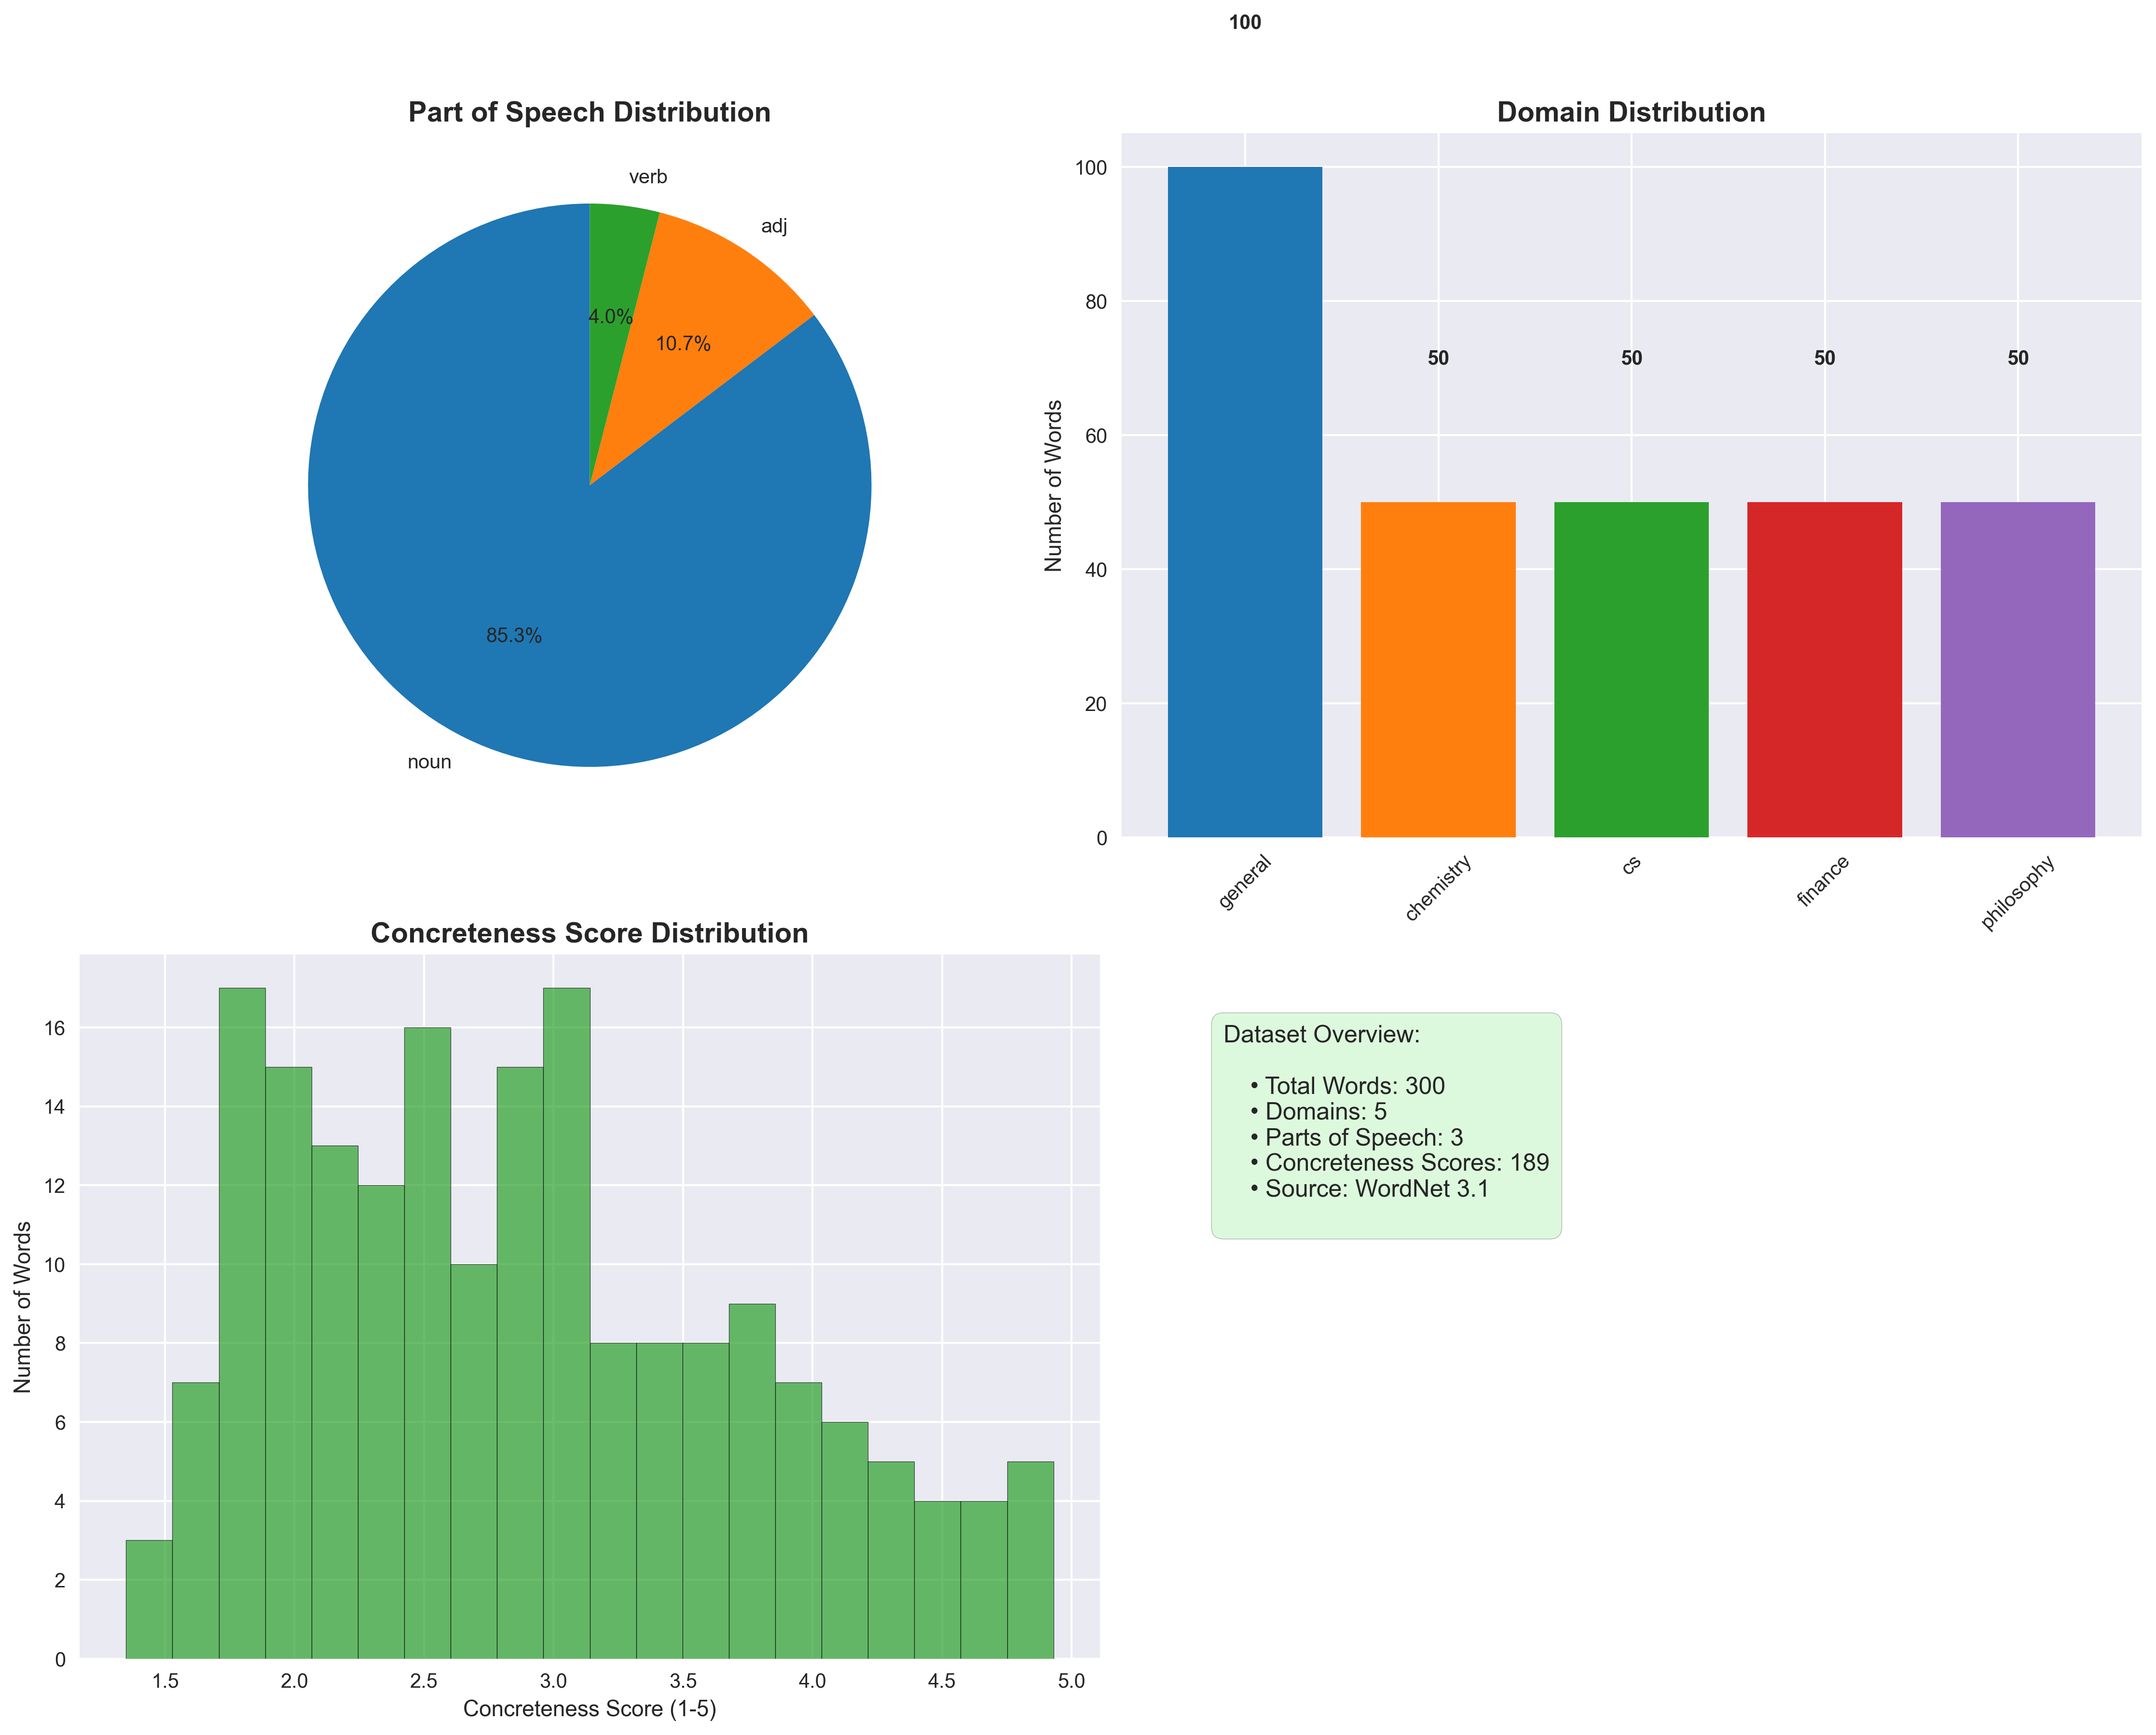
\includegraphics[width=\textwidth]{presentation_figures/figure2_dataset_distribution.png}
\end{center}
\end{column}
\end{columns}
\end{frame}

\begin{frame}{Evaluation Framework}
\begin{columns}[c]
\begin{column}{0.5\textwidth}
\begin{block}{Performance Metrics}
\begin{itemize}
    \item \textbf{Success Rate}: Games won
    \item \textbf{Efficiency}: Average turns
    \item \textbf{Turn 1 Success}: First-attempt rate
    \item \textbf{Rule Compliance}: Violation rate
\end{itemize}
\end{block}

\begin{block}{Statistical Methods}
Chi-square, correlation, ANOVA tests
\end{block}
\end{column}

\begin{column}{0.48\textwidth}
\begin{block}{Analysis Dimensions}
\begin{itemize}
    \item \textbf{Model Comparison}: Performance ranking
    \item \textbf{Linguistic Factors}: Frequency, POS, concreteness
    \item \textbf{Domain Effects}: Cross-domain variation
    \item \textbf{Error Analysis}: Failure patterns
\end{itemize}
\end{block}
\end{column}
\end{columns}
\end{frame}

%==============================================
% 3. Key Results
%==============================================
\section{Key Results}

% Section title slide
\begin{frame}
\begin{center}
\Huge \textbf{Key Results}
\end{center}
\end{frame}

\begin{frame}{Overall Model Performance}
\begin{columns}[c]
\begin{column}{0.5\textwidth}
\begin{block}{Performance Ranking}
\begin{center}
\begin{tabular}{lcc}
\toprule
\textbf{Model} & \textbf{Success Rate} & \textbf{Avg Turns} \\
\midrule
Gemini 2.5 Pro & 96.7\% & 1.6 \\
Claude Sonnet 4 & 95.9\% & 1.4 \\
DeepSeek Chat V3 & 89.4\% & 2.0 \\
GPT-4o & 80.5\% & 2.0 \\
\bottomrule
\end{tabular}
\end{center}
\end{block}

\begin{alertblock}{Major Finding}
Top two models significantly outperform bottom two, suggesting distinct capability tiers
\end{alertblock}
\end{column}

\begin{column}{0.48\textwidth}
\begin{center}
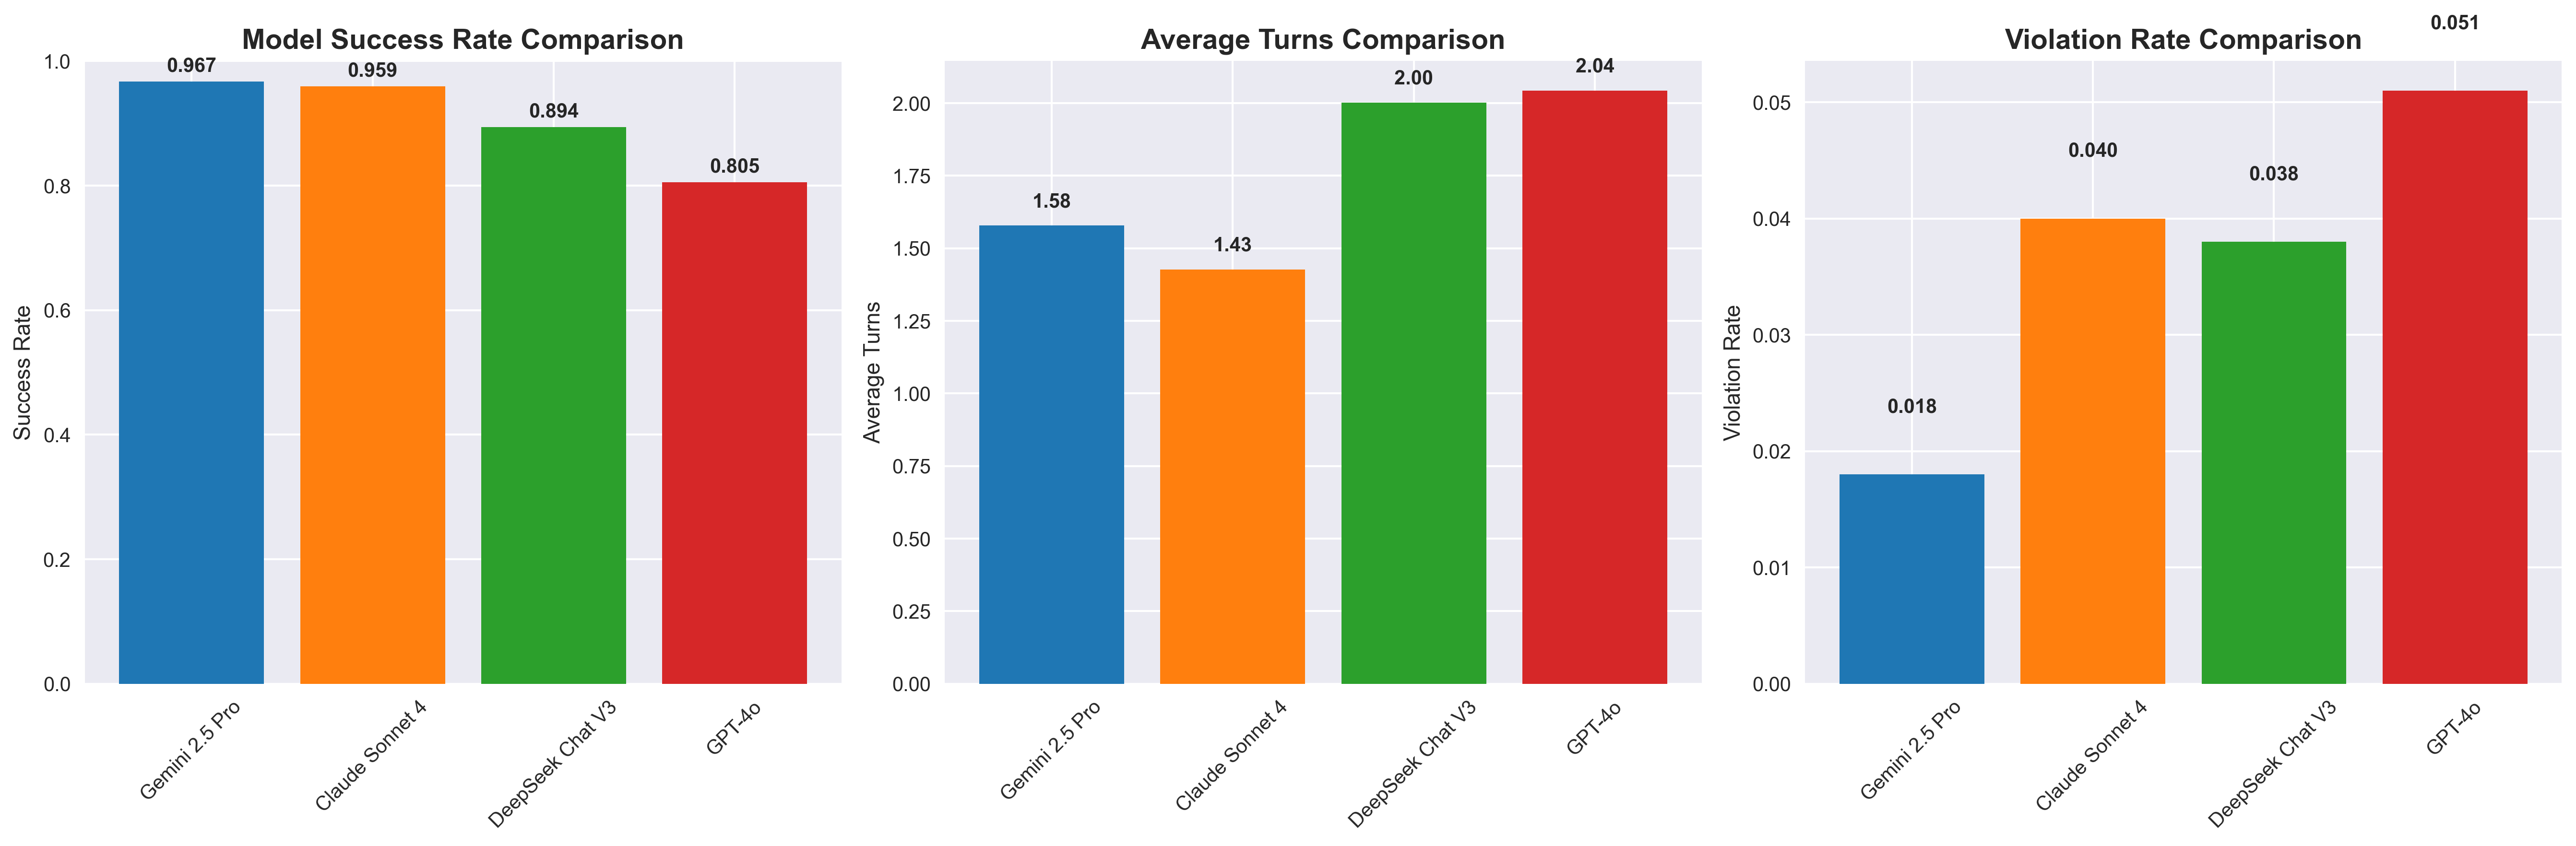
\includegraphics[width=\textwidth]{presentation_figures/figure3_model_performance.png}
\end{center}
\end{column}
\end{columns}
\end{frame}

\begin{frame}{Thinking Models vs Normal Models}
\begin{columns}[c]
\begin{column}{0.5\textwidth}
\begin{block}{Model Classification}
\begin{itemize}
    \item \textbf{Thinking Models}:
    \begin{itemize}
        \item Claude Sonnet 4
        \item Gemini 2.5 Pro
    \end{itemize}
    \item \textbf{Normal Models}:
    \begin{itemize}
        \item GPT-4o
        \item DeepSeek Chat V3
    \end{itemize}
\end{itemize}
\end{block}

\begin{block}{Performance Comparison}
\begin{center}
\begin{tabular}{lcc}
\toprule
\textbf{Type} & \textbf{Success Rate} & \textbf{Violation Rate} \\
\midrule
Thinking Models & 96.3\% & 2.9\% \\
Normal Models & 84.9\% & 4.5\% \\
\midrule
\textbf{Difference} & \textbf{+11.4\%} & \textbf{-1.6\%} \\
\bottomrule
\end{tabular}
\end{center}
\end{block}
\end{column}

\begin{column}{0.48\textwidth}
\begin{center}
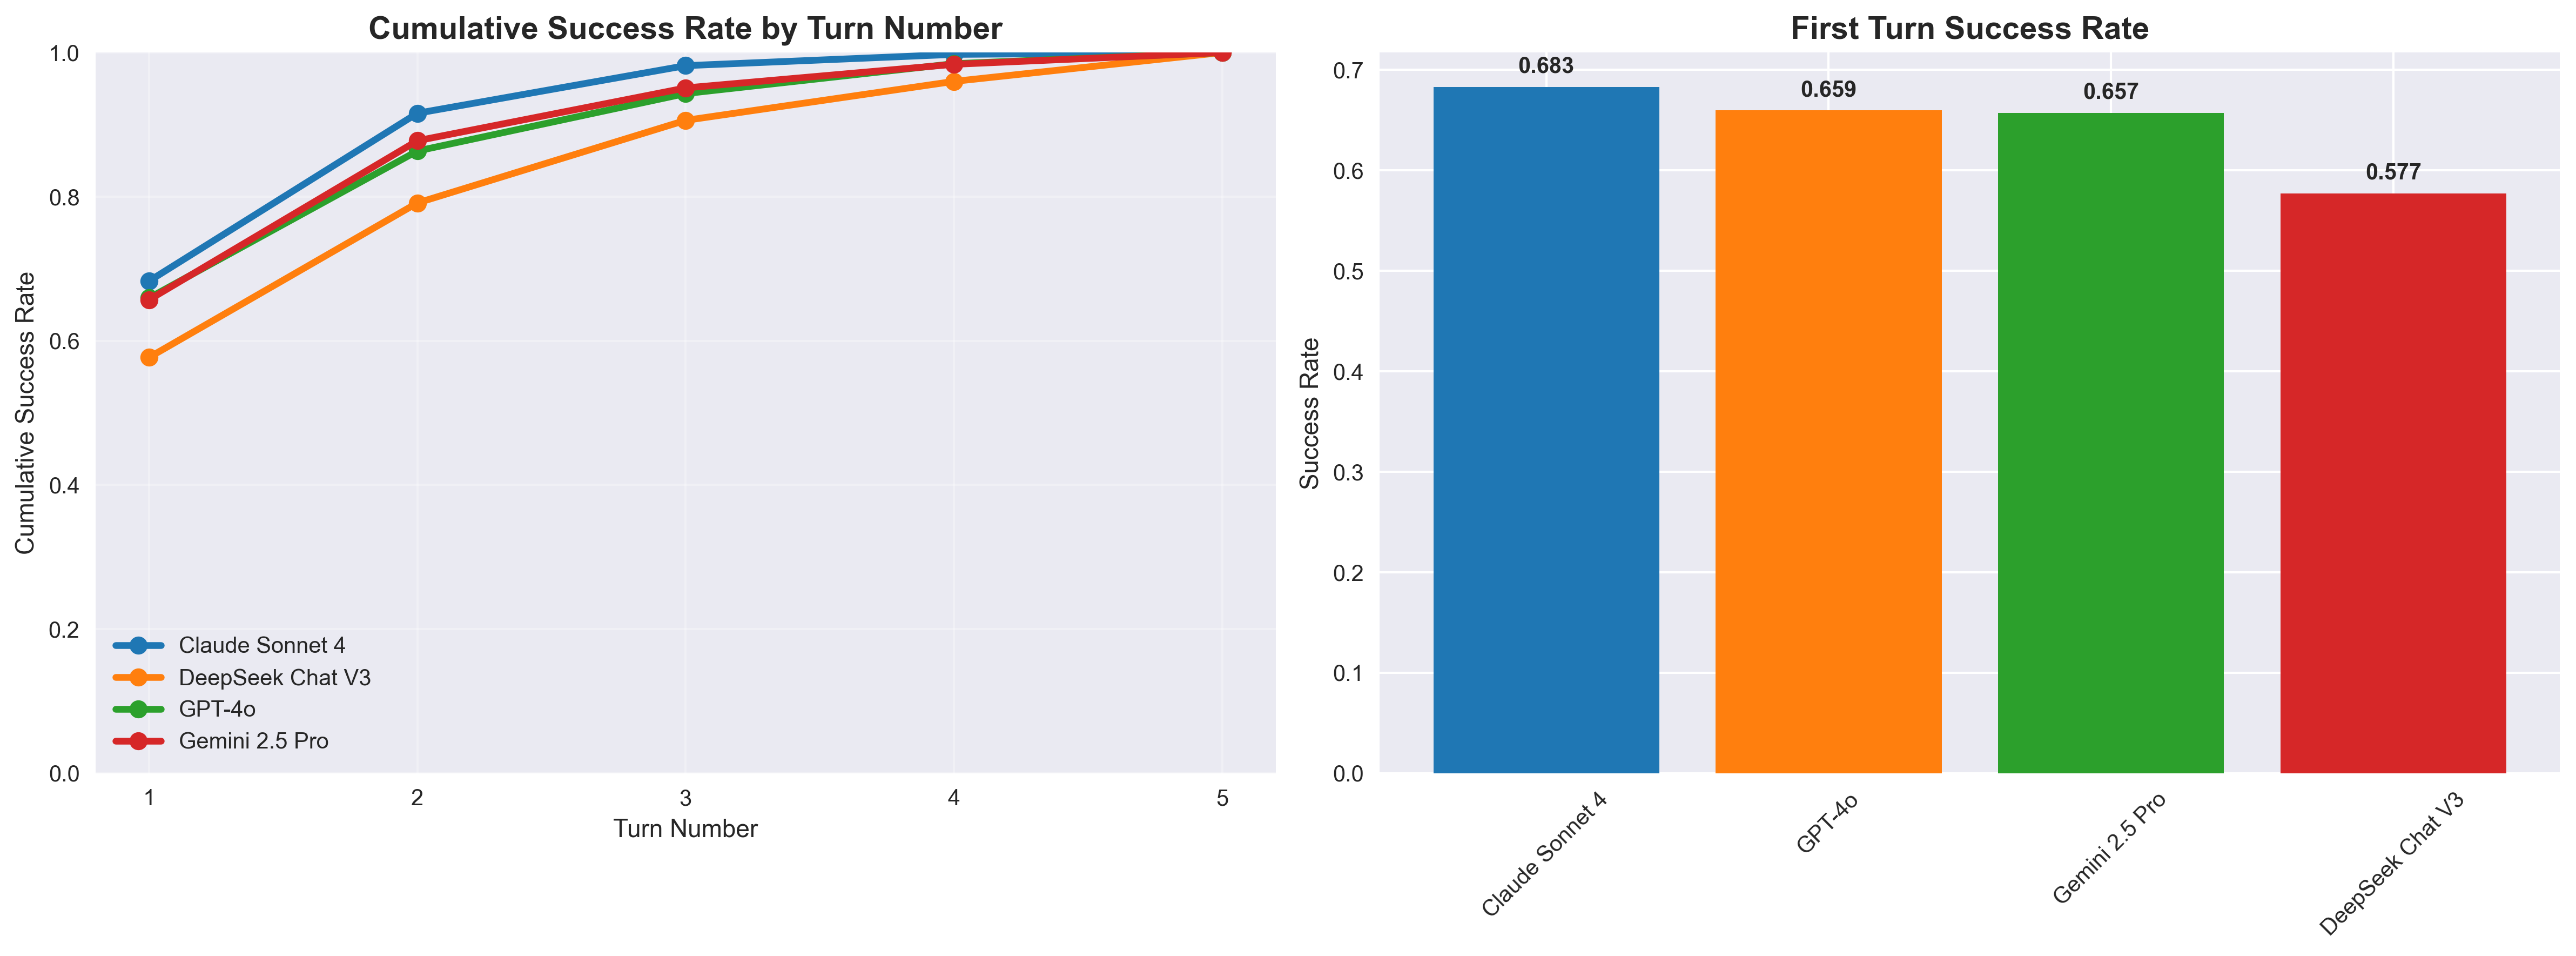
\includegraphics[width=\textwidth]{comprehensive_figures/figure2_efficiency.png}
\end{center}

\begin{alertblock}{Critical Discovery}
\small Thinking models show systematic advantages in efficiency and rule compliance
\end{alertblock}
\end{column}
\end{columns}
\end{frame}

\begin{frame}{Word Frequency Effects}
\begin{columns}[c]
\begin{column}{0.5\textwidth}
\begin{block}{Frequency Categories}
\begin{center}
\begin{tabular}{lcc}
\toprule
\textbf{Frequency} & \textbf{Success Rate} & \textbf{Games} \\
\midrule
Very Common & 97.7\% & 256 \\
Common & 94.9\% & 1,008 \\
Uncommon & 96.0\% & 1,312 \\
Rare & 93.1\% & 1,152 \\
Very Rare & 75.7\% & 1,072 \\
\bottomrule
\end{tabular}
 \end{center}
 \end{block}
 
 \begin{alertblock}{Major Discovery}
 Word frequency is a stronger predictor of performance than domain knowledge
 \end{alertblock}
 \end{column}
 
 \begin{column}{0.48\textwidth}
 \begin{center}
 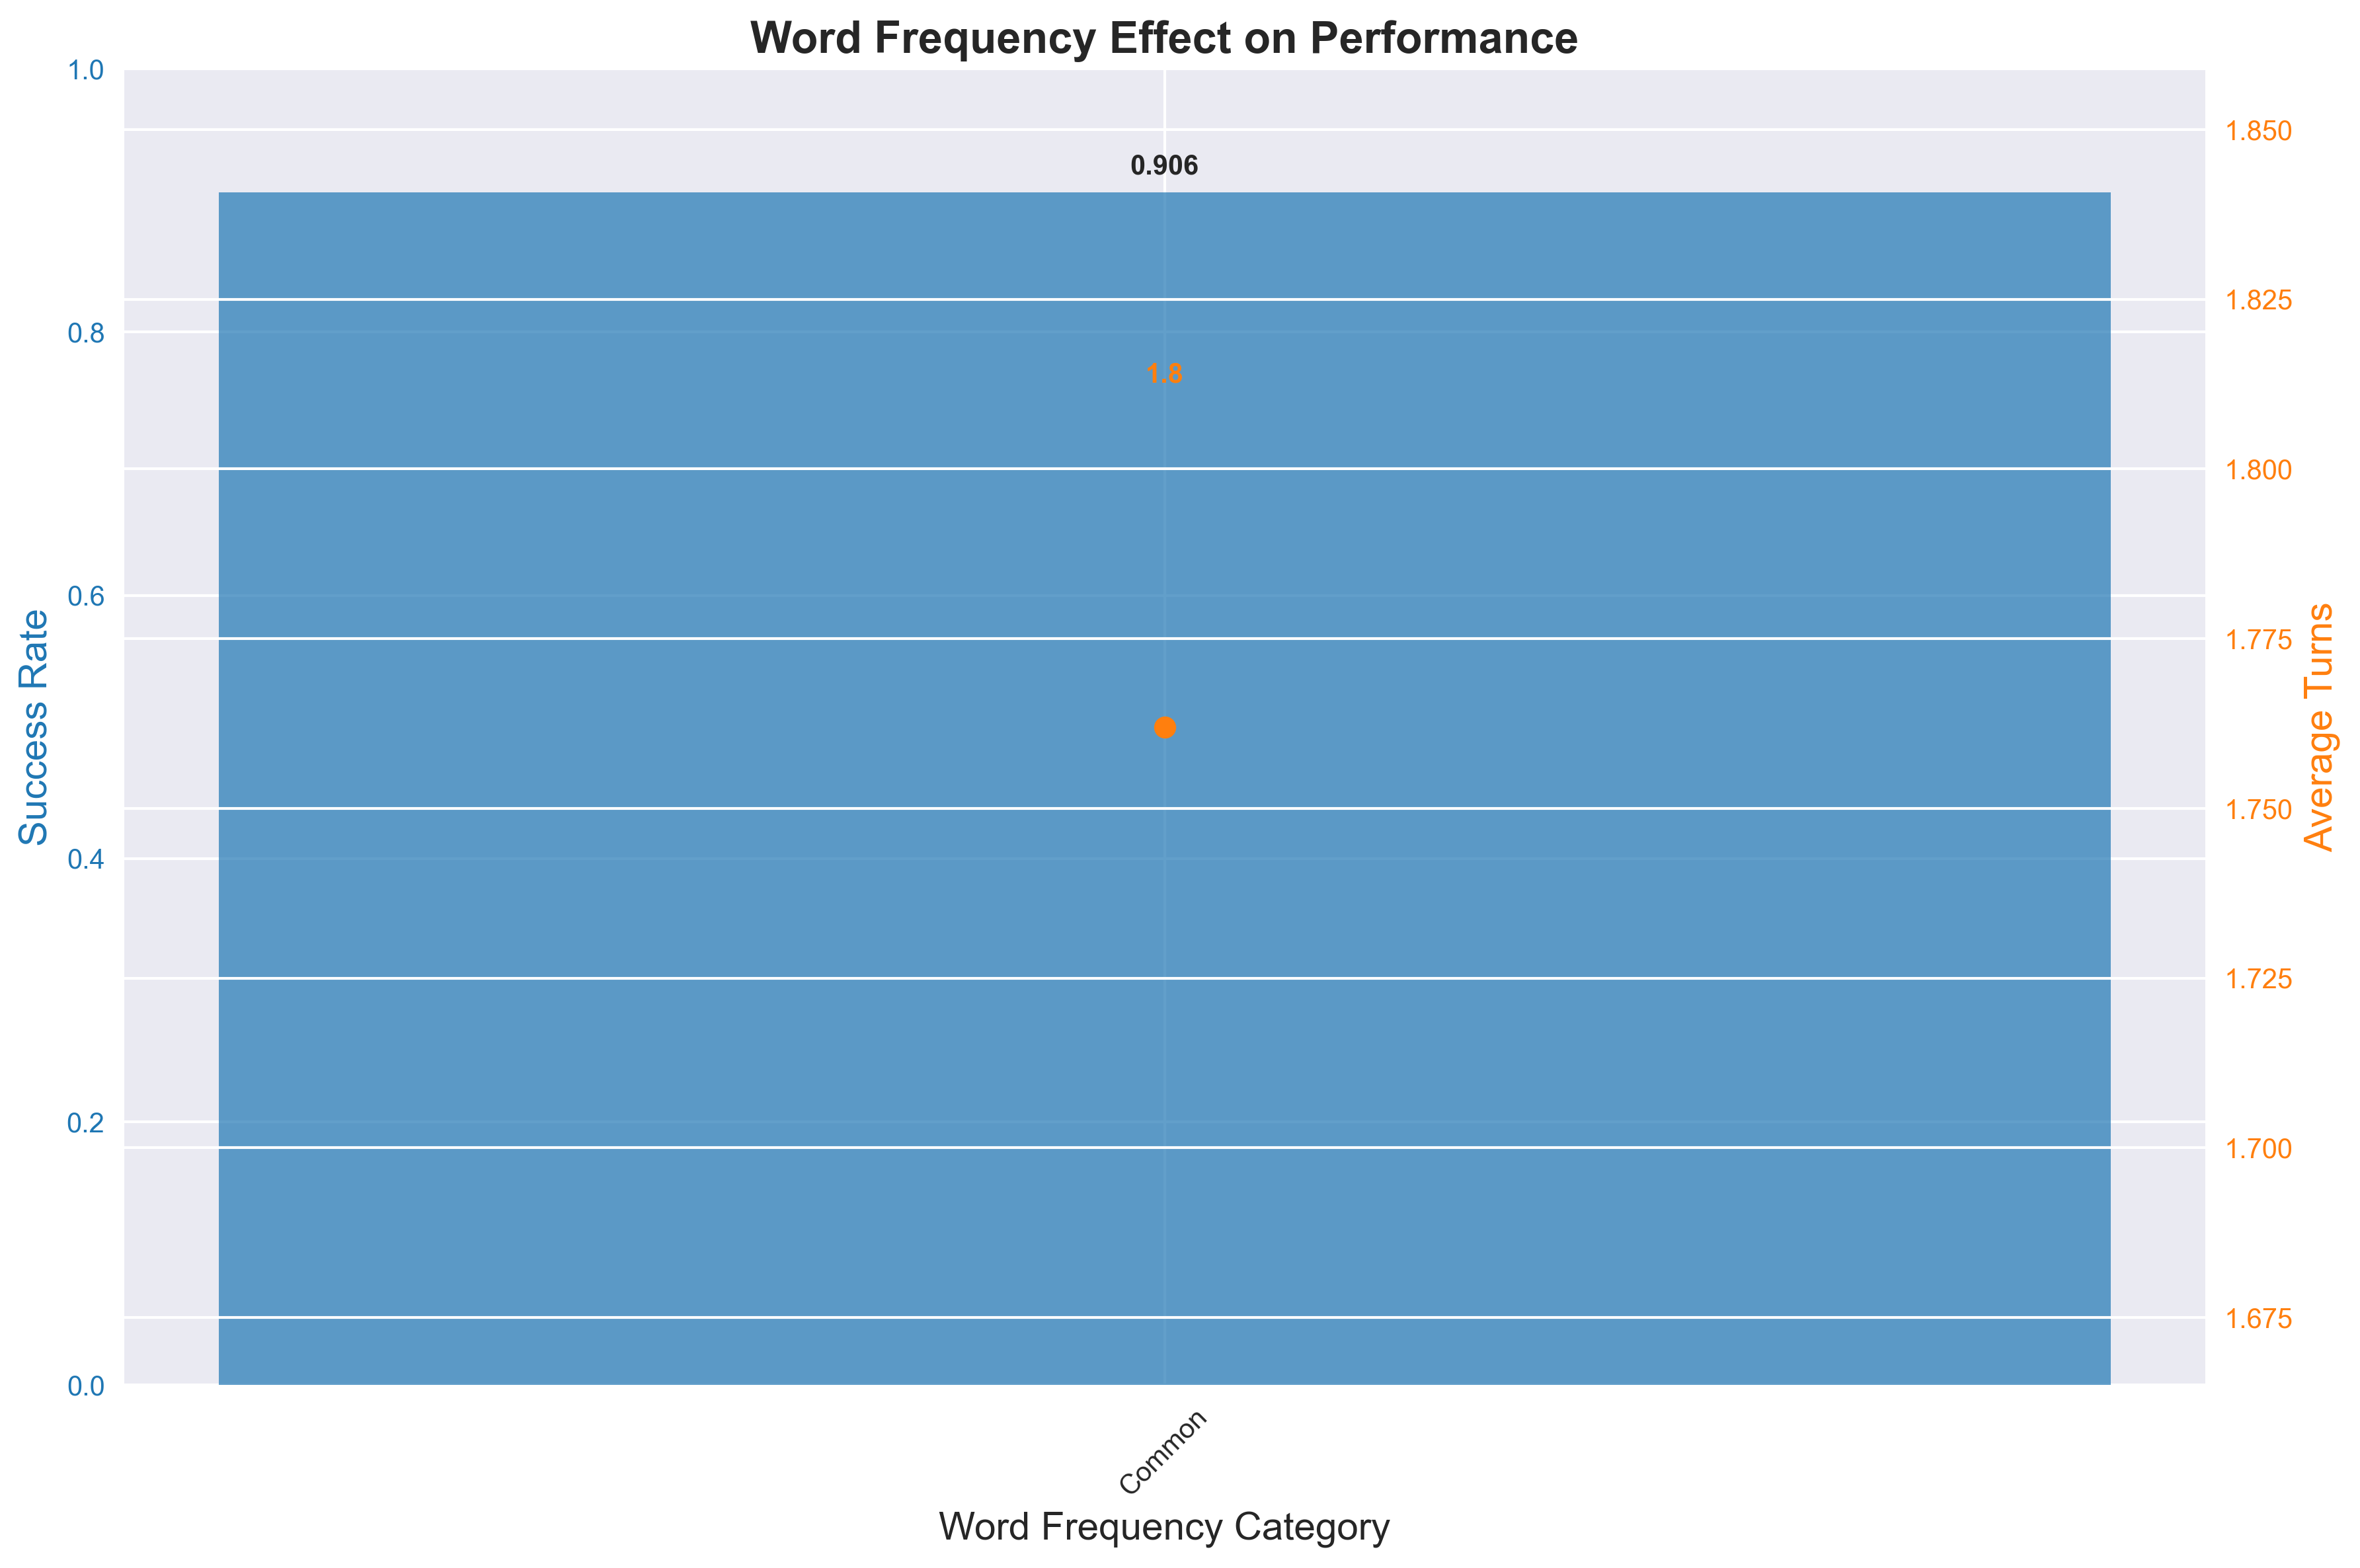
\includegraphics[width=\textwidth]{presentation_figures/figure5_frequency_effect.png}
 \end{center}
 \end{column}
 \end{columns}
 \end{frame}

\begin{frame}{Domain vs Frequency Effects}
\begin{columns}[c]
\begin{column}{0.5\textwidth}
\begin{block}{Apparent Domain Effects}
\begin{center}
\begin{tabular}{lc}
\toprule
\textbf{Domain} & \textbf{Success Rate} \\
\midrule
Finance & 98.2\% \\
Computer Science & 97.1\% \\
Philosophy & 92.6\% \\
Chemistry & 89.8\% \\
General & 83.0\% \\
\bottomrule
\end{tabular}
\end{center}
\end{block}

\begin{block}{Initial Interpretation}
\begin{itemize}
    \item Specialized domains outperform general
    \item Technical knowledge appears beneficial
    \item 15.2\% performance gap
\end{itemize}
\end{block}
\end{column}

\begin{column}{0.48\textwidth}
\begin{alertblock}{Critical Reanalysis}
When controlling for word frequency:
\begin{itemize}
    \item 65.9\% of domain effects disappear
    \item Frequency explains most variation
    \item True domain effects are minimal
\end{itemize}
\end{alertblock}

\begin{block}{Key Insight}
Word frequency is the primary performance factor
\end{block}
\end{column}
\end{columns}
\end{frame}

\begin{frame}{Linguistic Factors Analysis}
\begin{columns}[c]
\begin{column}{0.5\textwidth}
\begin{block}{Part-of-Speech Effects}
\begin{center}
\begin{tabular}{lcc}
\toprule
\textbf{POS} & \textbf{Success Rate} & \textbf{Difficulty} \\
\midrule
Noun & 92.0\% & Easiest \\
Verb & 87.5\% & Medium \\
Adjective & 81.1\% & Hardest \\
\bottomrule
\end{tabular}
\end{center}
\end{block}

\begin{block}{Concreteness Effects}
\begin{itemize}
    \item \textbf{Concrete words}: 92.4\% success
    \item \textbf{Abstract words}: 84.7\% success
    \item \textbf{Difference}: 7.7 percentage points (p < 0.01)
\end{itemize}
\end{block}
\end{column}

\begin{column}{0.48\textwidth}
\begin{center}
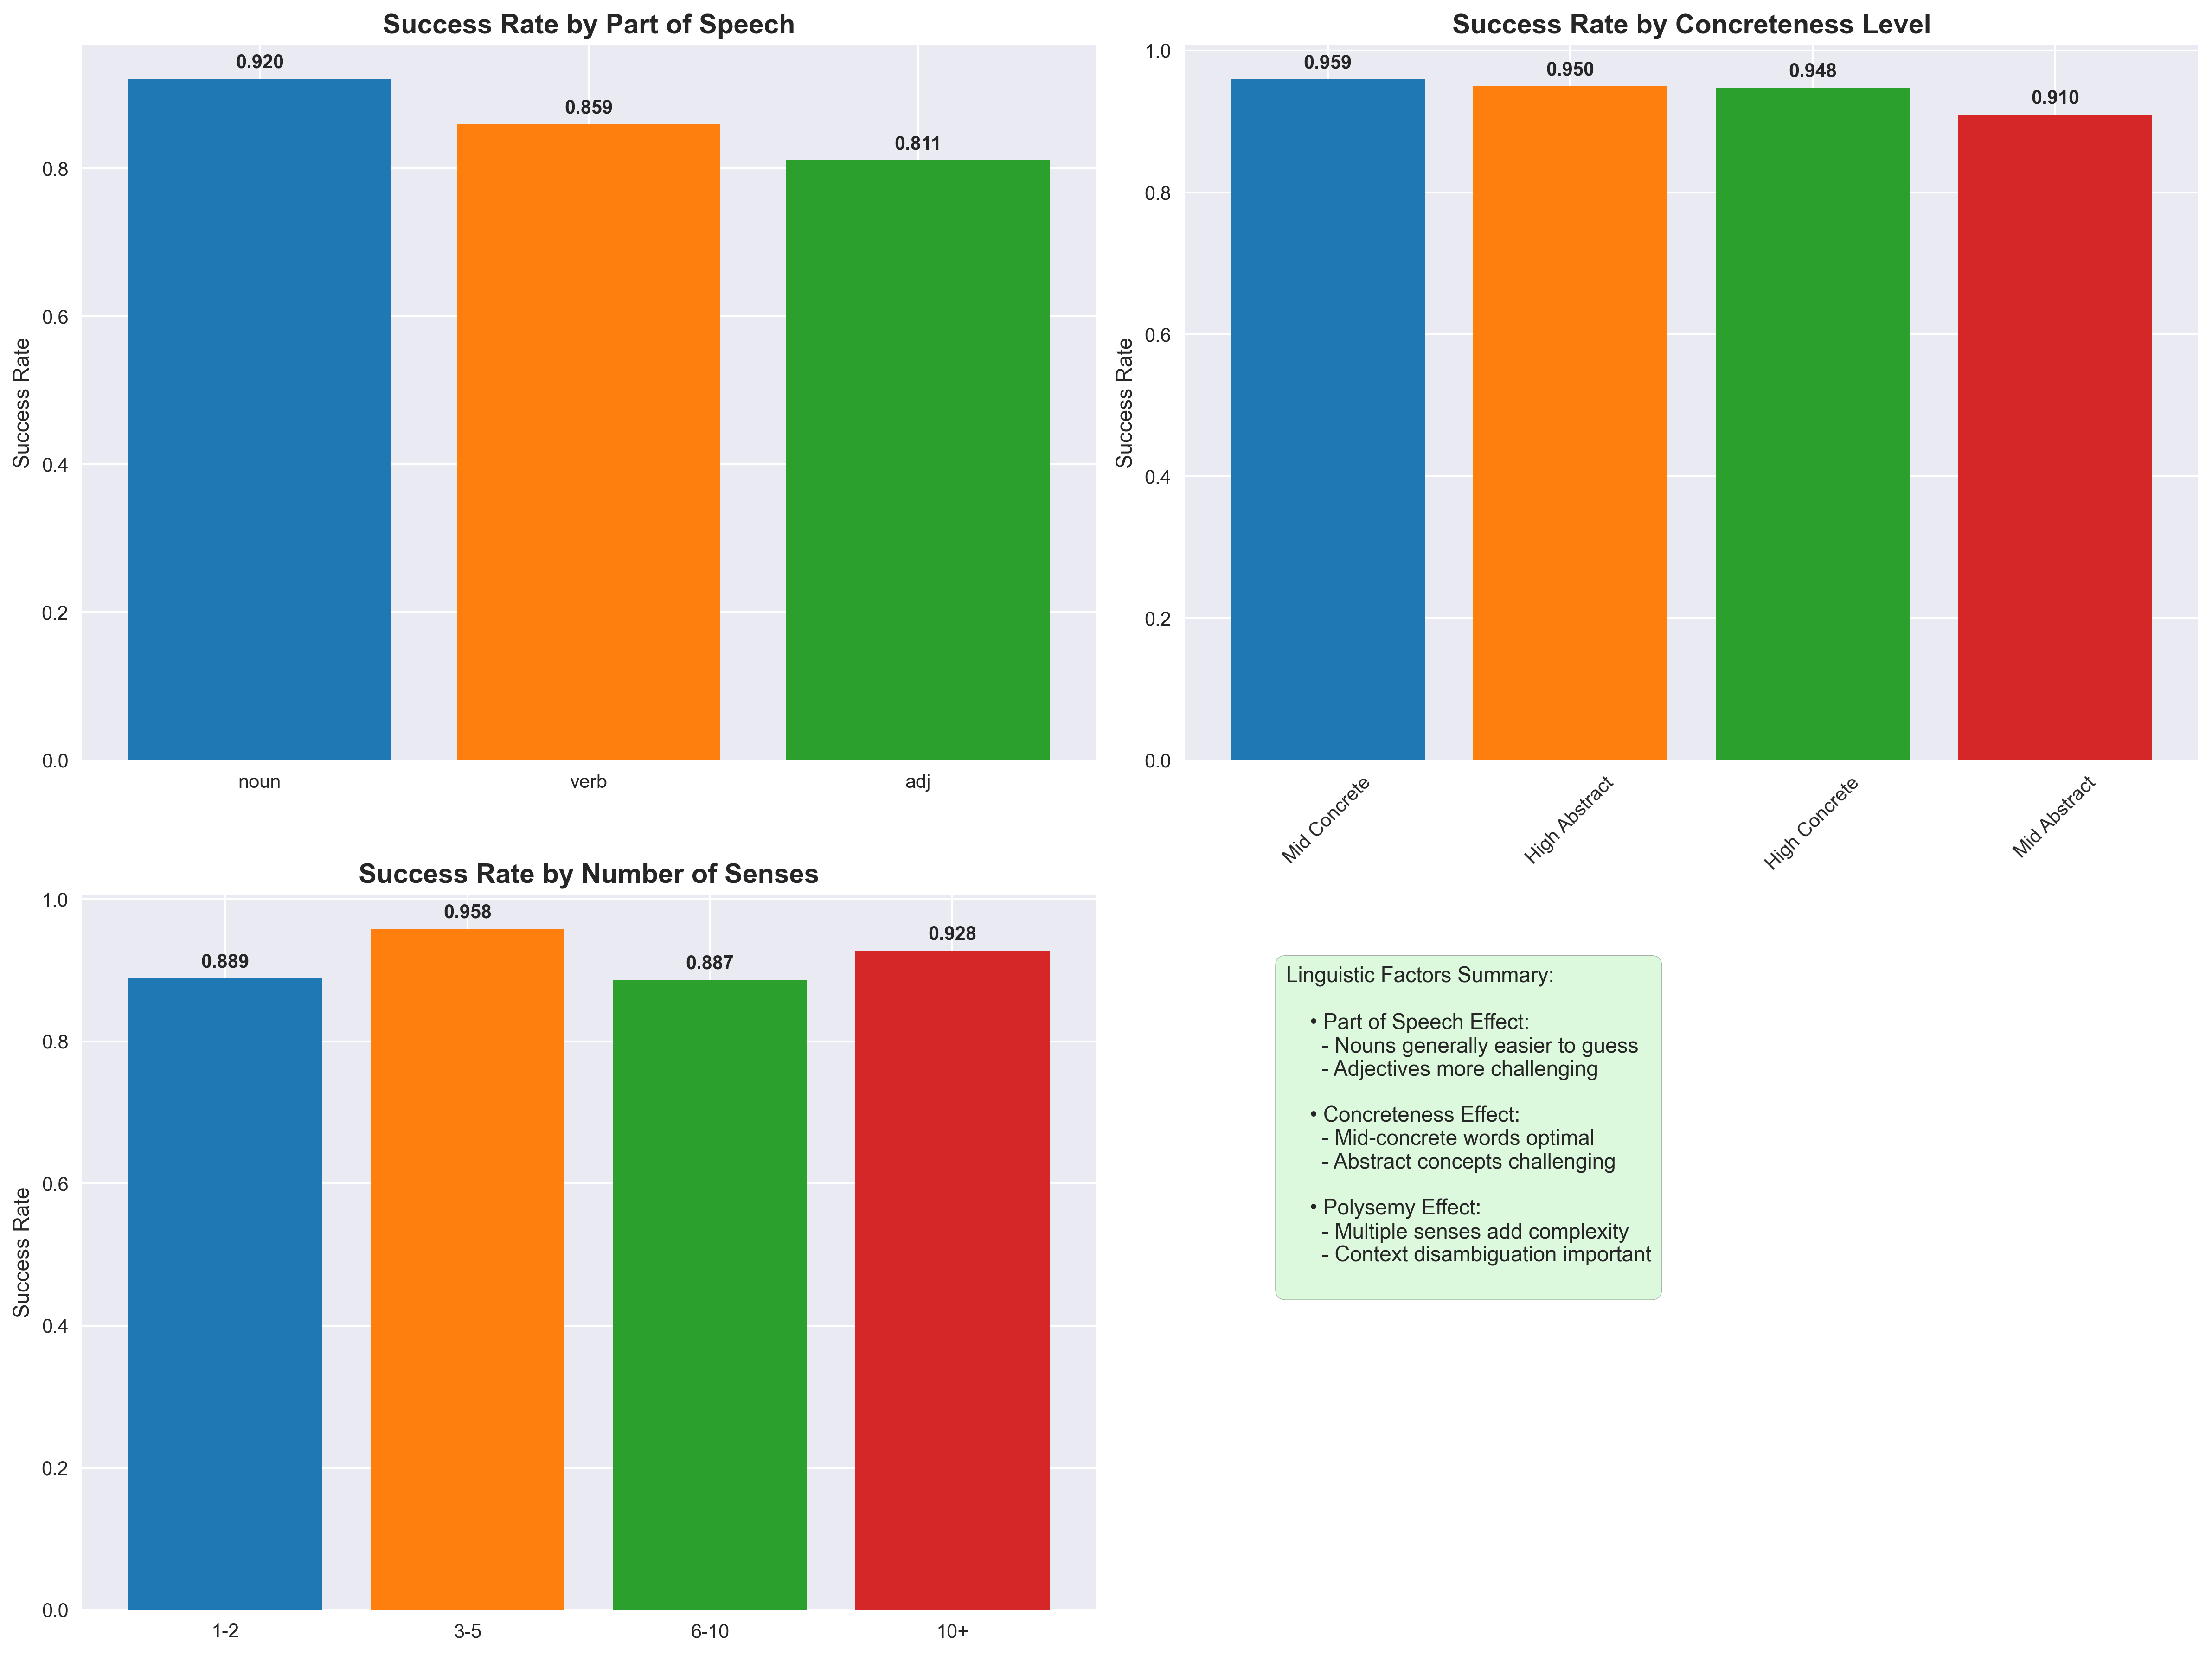
\includegraphics[width=\textwidth]{comprehensive_figures/figure3_linguistic.png}
\end{center}
\end{column}
\end{columns}
\end{frame}

\begin{frame}{Error Analysis}
\begin{columns}[c]
\begin{column}{0.5\textwidth}
\begin{block}{Failure Reasons}
\begin{center}
\begin{tabular}{lcc}
\toprule
\textbf{Failure Type} & \textbf{Count} & \textbf{\%} \\
\midrule
Max Turns Exceeded & 234 & 52.0\% \\
Taboo Violation & 177 & 39.3\% \\
Format Error & 39 & 8.7\% \\
\bottomrule
\end{tabular}
\end{center}
\end{block}

\begin{block}{Model-Specific Patterns}
\begin{itemize}
    \item GPT-4o: Highest violation rate (5.1\%)
    \item Gemini: Lowest violation rate (1.8\%)
    \item Claude: Best efficiency (1.4 turns)
\end{itemize}
\end{block}
\end{column}

\begin{column}{0.48\textwidth}
\begin{block}{Error Insights}
\begin{itemize}
    \item Most failures due to difficulty, not rule violations
    \item Constraint adherence varies significantly
    \item Format errors minimal with clear instructions
\end{itemize}
\end{block}

\begin{block}{Improvement Opportunities}
\begin{itemize}
    \item Better constraint instruction methods
    \item Adaptive turn limits
    \item Enhanced rule compliance training
\end{itemize}
\end{block}
\end{column}
\end{columns}
\end{frame}

%==============================================
% 4. Key Findings
%==============================================
\section{Key Findings}

% Section title slide
\begin{frame}
\begin{center}
\Huge \textbf{Key Findings}
\end{center}
\end{frame}

\begin{frame}{Major Discoveries}
\begin{alertblock}{1. Thinking Model Superiority}
Thinking models systematically outperform normal models by 11.4\% in success rate
\end{alertblock}

\begin{alertblock}{2. Frequency Dominance}
Word frequency explains 65.9\% of apparent domain effects (r = 0.225, p < 0.001)
\end{alertblock}

\begin{alertblock}{3. Performance Hierarchy}
Clear model ranking: Gemini $\approx$ Claude >> DeepSeek > GPT-4o
\end{alertblock}

\begin{block}{Secondary Findings}
\begin{itemize}
    \item Nouns easier than adjectives
    \item Concrete words outperform abstract words
    \item Rule compliance varies significantly across models
\end{itemize}
\end{block}
\end{frame}

\begin{frame}{Theoretical Implications}
\begin{block}{For AI Research}
\begin{itemize}
    \item Internal reasoning mechanisms matter for constrained tasks
    \item Training data frequency distribution critically affects performance
    \item Domain specialization claims may be overestimated
    \item Constraint-following capabilities require specific attention
\end{itemize}
\end{block}

\begin{block}{For Cognitive Science}
\begin{itemize}
    \item LLMs exhibit human-like frequency effects
    \item Creative language generation follows predictable patterns
    \item Constrained communication reveals linguistic flexibility limits
\end{itemize}
\end{block}

\begin{block}{For Practical Applications}
\small
\begin{itemize}
    \item Model selection depends on constraint requirements
    \item Vocabulary frequency guides evaluation design
    \item Thinking models preferred for rule-sensitive tasks
\end{itemize}
\end{block}
\end{frame}

%==============================================
% 5. Challenges & Solutions
%==============================================
\section{Challenges \& Solutions}

% Section title slide
\begin{frame}
\begin{center}
\Huge \textbf{Challenges \& Solutions}
\end{center}
\end{frame}

\begin{frame}{Technical Challenges}
\begin{block}{API and Infrastructure Issues}
\begin{itemize}
    \item \textbf{Challenge}: Rate limits and cost management
    \item \textbf{Solution}: Batch processing, async requests, retry mechanisms
\end{itemize}
\end{block}

\begin{block}{Data Quality Control}
\begin{itemize}
    \item \textbf{Challenge}: Detecting taboo word violations
    \item \textbf{Solution}: Automated checking + manual validation
\end{itemize}
\end{block}

\begin{block}{Evaluation Consistency}
\begin{itemize}
    \item \textbf{Challenge}: Subjective success determination
    \item \textbf{Solution}: Clear criteria, multiple evaluators, statistical validation
\end{itemize}
\end{block}

\begin{block}{Scale Management}
\small
\begin{itemize}
    \item \textbf{Challenge}: 4,800 games across 4 models
    \item \textbf{Solution}: Automated pipeline, error handling
\end{itemize}
\end{block}
\end{frame}

\begin{frame}{Methodological Improvements}
\begin{block}{Initial Approach Limitations}
\begin{itemize}
    \item Simple binary success/failure metrics
    \item Limited linguistic feature analysis
    \item Basic statistical comparisons
\end{itemize}
\end{block}

\begin{block}{Enhanced Framework}
\begin{itemize}
    \item Multi-dimensional performance metrics
    \item Comprehensive linguistic feature integration
    \item Advanced statistical analysis (ANOVA, correlation, effect sizes)
    \item Systematic error pattern analysis
\end{itemize}
\end{block}

\begin{block}{Quality Assurance}
\small
\begin{itemize}
    \item Reproducible experimental protocols
    \item Statistical significance testing
    \item Cross-validation of key findings
\end{itemize}
\end{block}
\end{frame}

%==============================================
% 6. Current Progress & Next Steps
%==============================================
\section{Current Progress \& Next Steps}

% Section title slide
\begin{frame}
\begin{center}
\Huge \textbf{Current Progress \& Next Steps}
\end{center}
\end{frame}

\begin{frame}{Project Timeline \& Status}
\begin{block}{Completed Work (\checkmark)}
\begin{itemize}
    \item $\checkmark$ Literature review and methodology design
    \item $\checkmark$ Dataset construction and validation (300 words)
    \item $\checkmark$ Experimental framework implementation
    \item $\checkmark$ Data collection (4,800 games across 4 models)
    \item $\checkmark$ Core statistical analysis and visualization
    \item $\checkmark$ Major findings identification
\end{itemize}
\end{block}

\begin{block}{Current Status}
\begin{itemize}
    \item \textbf{90\% complete}: Main analysis and results
    \item \textbf{In progress}: Deep dive analysis and validation
    \item \textbf{Starting}: Thesis writing and documentation
\end{itemize}
\end{block}
\end{frame}

\begin{frame}{Remaining Work Plan}
\begin{block}{Short-term (Next 4-6 weeks)}
\begin{itemize}
    \item Finalize supplementary analysis
    \item Validate key findings through additional testing
    \item Begin thesis writing (methodology and results chapters)
    \item Prepare code and data for reproducibility
\end{itemize}
\end{block}

\begin{block}{Medium-term (Following 6-8 weeks)}
\begin{itemize}
    \item Complete thesis writing
    \item Conduct final review and validation
    \item Prepare conference paper submission
    \item Develop open-source evaluation framework
\end{itemize}
\end{block}

\begin{block}{Risk Mitigation}
\small
\begin{itemize}
    \item Core results already validated and robust
    \item Backup analysis approaches prepared
    \item Time buffer built into schedule
\end{itemize}
\end{block}
\end{frame}

\begin{frame}{Expected Final Deliverables}
\begin{block}{Academic Outcomes}
\begin{itemize}
    \item \textbf{MSc Thesis}: Comprehensive 80-100 page document
    \item \textbf{Conference Paper}: Target venue submission
    \item \textbf{Evaluation Framework}: Reusable methodology for future research
\end{itemize}
\end{block}

\begin{block}{Practical Contributions}
\begin{itemize}
    \item \textbf{Open Dataset}: 300-word Taboo evaluation set
    \item \textbf{Code Repository}: Complete experimental pipeline
    \item \textbf{Performance Benchmarks}: Baseline results for 4 LLMs
    \item \textbf{Best Practices}: Guidelines for constraint-based evaluation
\end{itemize}
\end{block}

\begin{block}{Impact Potential}
\small
\begin{itemize}
    \item Advance LLM evaluation methodologies
    \item Inform model selection for constraint-sensitive apps
    \item Contribute to AI creativity and rule-following understanding
\end{itemize}
\end{block}
\end{frame}

%==============================================
% 7. Conclusion
%==============================================
\section{Conclusion}

% Section title slide
\begin{frame}
\begin{center}
\Huge \textbf{Conclusion}
\end{center}
\end{frame}

\begin{frame}{Project Summary}
\begin{columns}[c]
\begin{column}{0.5\textwidth}
\begin{block}{What We've Accomplished}
\begin{itemize}
    \item \textbf{Methodological Innovation}: First systematic Taboo game evaluation for LLMs
    \item \textbf{Empirical Discoveries}: Thinking model advantages, frequency dominance
    \item \textbf{Comprehensive Analysis}: Multi-dimensional performance assessment
    \item \textbf{Practical Insights}: Model selection guidance and optimization strategies
\end{itemize}
\end{block}

\begin{alertblock}{Research Impact}
This work establishes foundation for more reliable and controllable AI systems through better understanding of constraint-following capabilities
\end{alertblock}
\end{column}

\begin{column}{0.48\textwidth}
\begin{center}
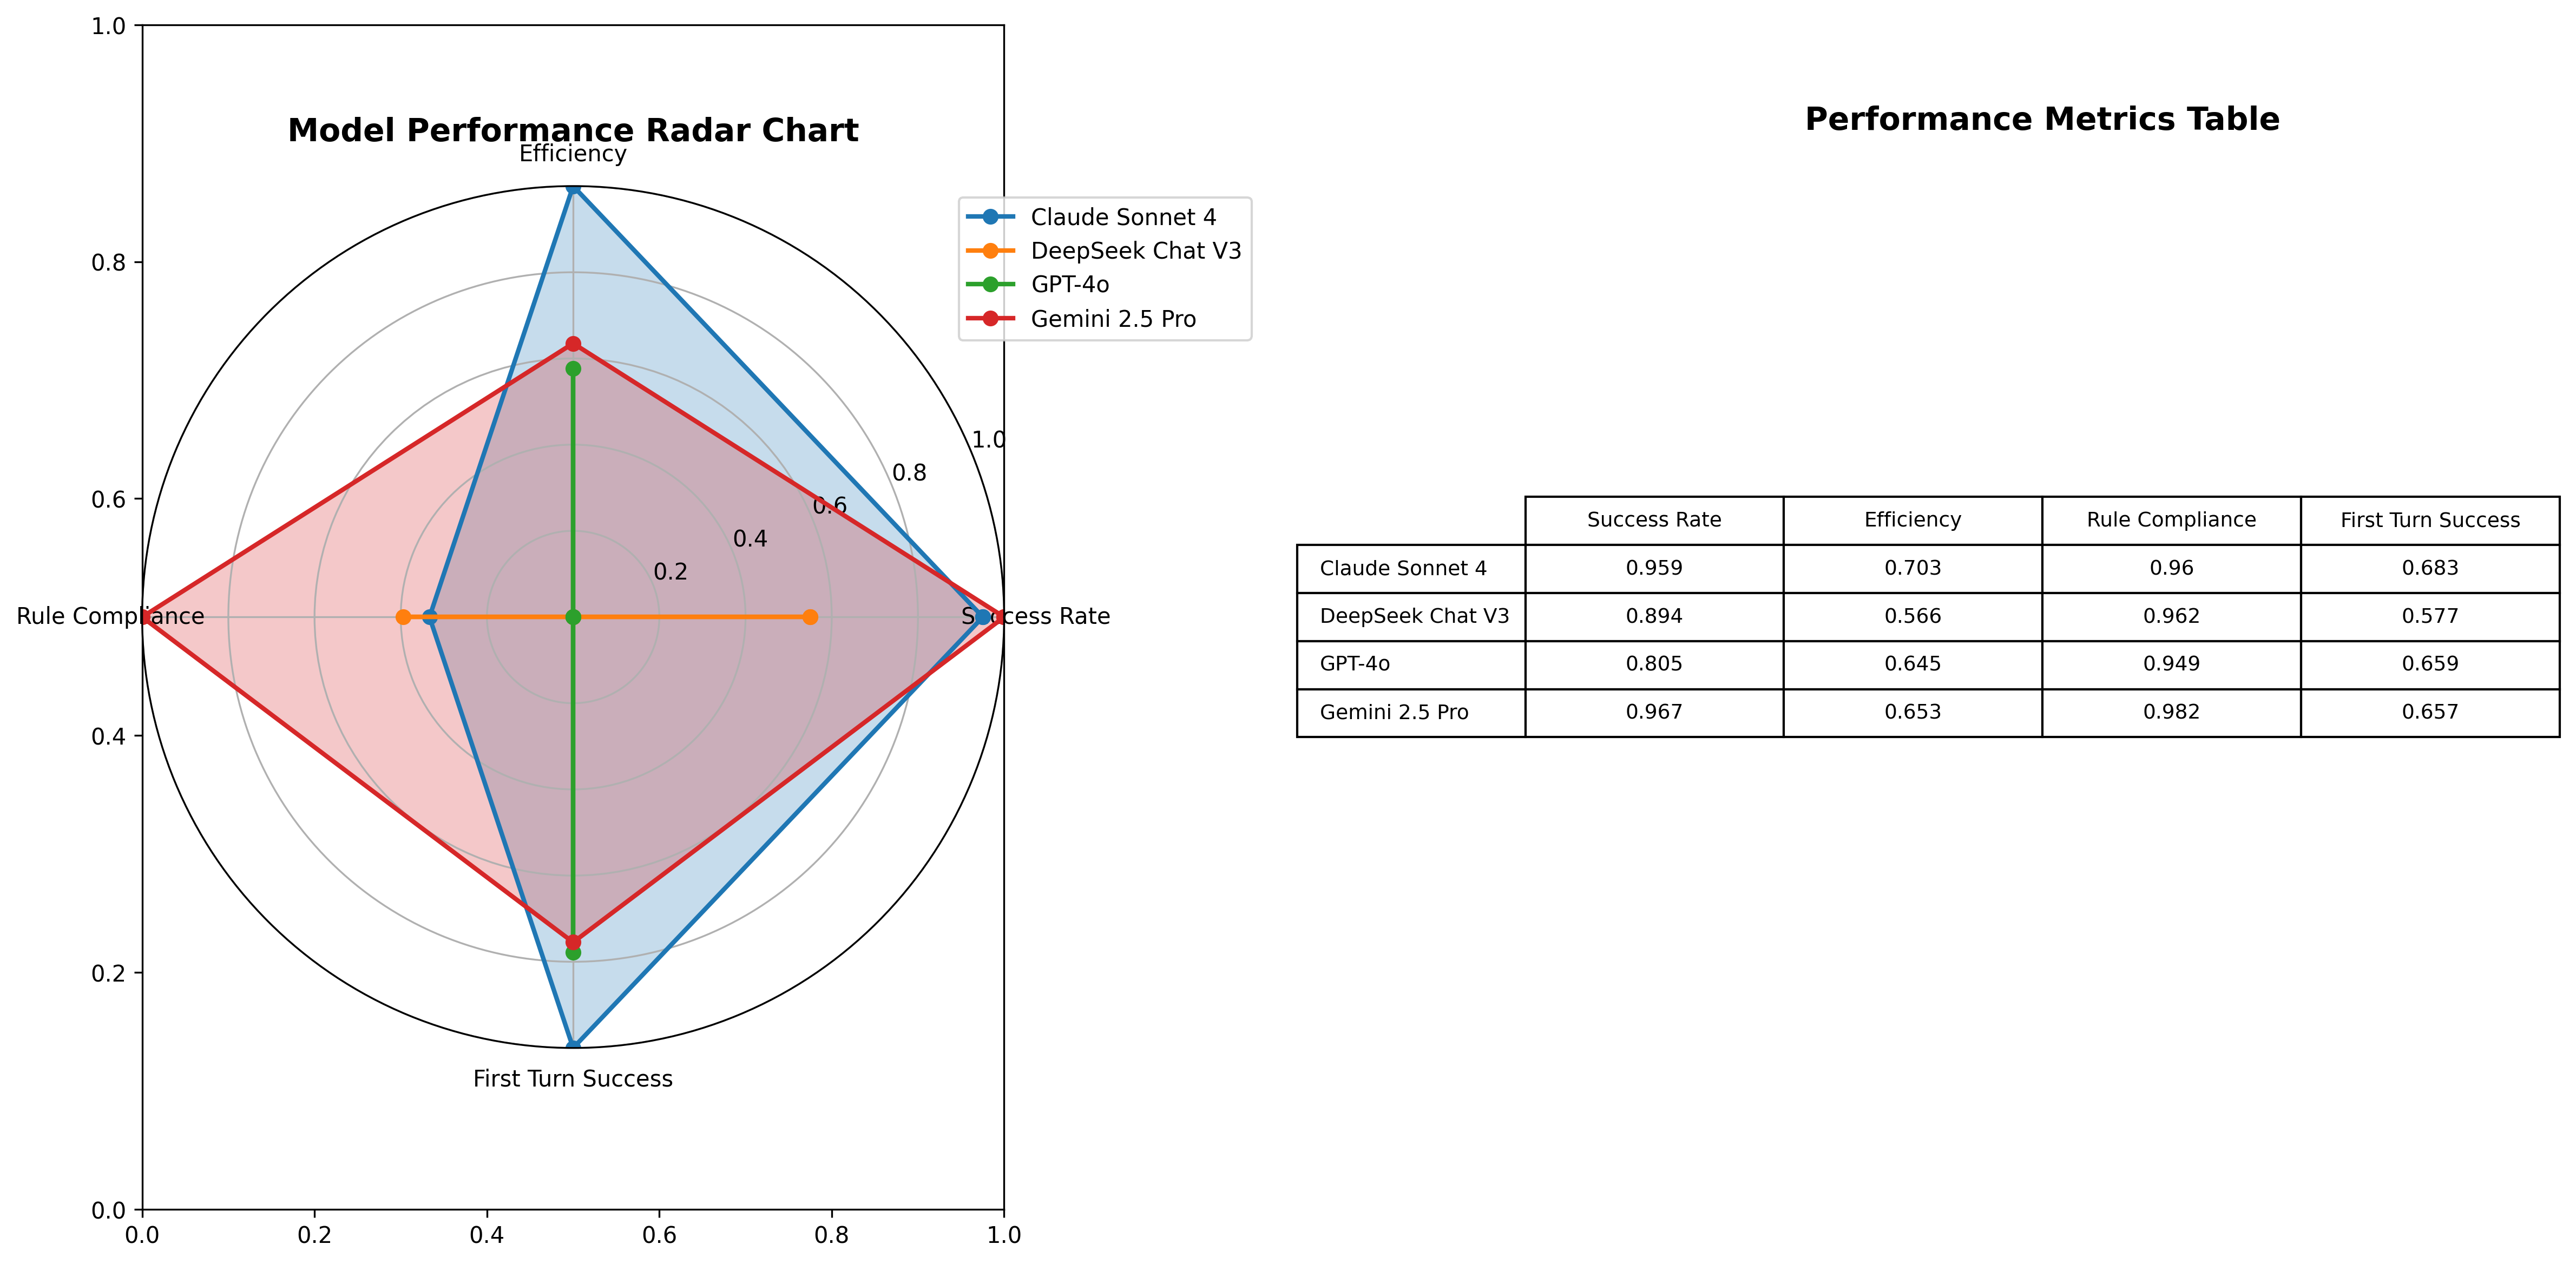
\includegraphics[width=\textwidth]{comprehensive_figures/figure7_radar.png}
\end{center}
\end{column}
\end{columns}
\end{frame}

\begin{frame}{Looking Forward}
\begin{block}{Immediate Applications}
\begin{itemize}
    \item Model selection guidance for constraint-sensitive tasks
    \item Training data optimization recommendations
    \item Evaluation methodology improvements
    \item Benchmark establishment for future research
\end{itemize}
\end{block}

\begin{block}{Future Research Directions}
\begin{itemize}
    \item Expand to multilingual evaluation
    \item Test additional model architectures
    \item Investigate fine-tuning for constraint adherence
    \item Explore other constrained generation tasks
\end{itemize}
\end{block}

\begin{block}{Project Confidence}
\small
\begin{itemize}
    \item Strong empirical foundation with 4,800 data points
    \item Multiple validated findings with statistical significance
    \item Clear path to completion within timeline
    \item High potential for impactful contributions
\end{itemize}
\end{block}
\end{frame}

% Thank you slide
\begin{frame}[plain]
\begin{center}
\huge Thank You!

\vspace{1cm}

\Large Questions \& Discussion

\vspace{1cm}

\normalsize
\textbf{Contact:} student.email@university.edu\\
\textbf{Project Repository:} github.com/username/taboo-llm-eval\\
\textbf{Progress Updates:} [Project Website/Blog]
\end{center}
\end{frame}

\end{document} 